\documentclass[1p]{elsarticle_modified}
%\bibliographystyle{elsarticle-num}

%\usepackage[colorlinks]{hyperref}
%\usepackage{abbrmath_seonhwa} %\Abb, \Ascr, \Acal ,\Abf, \Afrak
\usepackage{amsfonts}
\usepackage{amssymb}
\usepackage{amsmath}
\usepackage{amsthm}
\usepackage{scalefnt}
\usepackage{amsbsy}
\usepackage{kotex}
\usepackage{caption}
\usepackage{subfig}
\usepackage{color}
\usepackage{graphicx}
\usepackage{xcolor} %% white, black, red, green, blue, cyan, magenta, yellow
\usepackage{float}
\usepackage{setspace}
\usepackage{hyperref}

\usepackage{tikz}
\usetikzlibrary{arrows}

\usepackage{multirow}
\usepackage{array} % fixed length table
\usepackage{hhline}

%%%%%%%%%%%%%%%%%%%%%
\makeatletter
\renewcommand*\env@matrix[1][\arraystretch]{%
	\edef\arraystretch{#1}%
	\hskip -\arraycolsep
	\let\@ifnextchar\new@ifnextchar
	\array{*\c@MaxMatrixCols c}}
\makeatother %https://tex.stackexchange.com/questions/14071/how-can-i-increase-the-line-spacing-in-a-matrix
%%%%%%%%%%%%%%%

\usepackage[normalem]{ulem}

\newcommand{\msout}[1]{\ifmmode\text{\sout{\ensuremath{#1}}}\else\sout{#1}\fi}
%SOURCE: \msout is \stkout macro in https://tex.stackexchange.com/questions/20609/strikeout-in-math-mode

\newcommand{\cancel}[1]{
	\ifmmode
	{\color{red}\msout{#1}}
	\else
	{\color{red}\sout{#1}}
	\fi
}

\newcommand{\add}[1]{
	{\color{blue}\uwave{#1}}
}

\newcommand{\replace}[2]{
	\ifmmode
	{\color{red}\msout{#1}}{\color{blue}\uwave{#2}}
	\else
	{\color{red}\sout{#1}}{\color{blue}\uwave{#2}}
	\fi
}

\newcommand{\Sol}{\mathcal{S}} %segment
\newcommand{\D}{D} %diagram
\newcommand{\A}{\mathcal{A}} %arc


%%%%%%%%%%%%%%%%%%%%%%%%%%%%%5 test

\def\sl{\operatorname{\textup{SL}}(2,\Cbb)}
\def\psl{\operatorname{\textup{PSL}}(2,\Cbb)}
\def\quan{\mkern 1mu \triangleright \mkern 1mu}

\theoremstyle{definition}
\newtheorem{thm}{Theorem}[section]
\newtheorem{prop}[thm]{Proposition}
\newtheorem{lem}[thm]{Lemma}
\newtheorem{ques}[thm]{Question}
\newtheorem{cor}[thm]{Corollary}
\newtheorem{defn}[thm]{Definition}
\newtheorem{exam}[thm]{Example}
\newtheorem{rmk}[thm]{Remark}
\newtheorem{alg}[thm]{Algorithm}

\newcommand{\I}{\sqrt{-1}}
\begin{document}

%\begin{frontmatter}
%
%\title{Boundary parabolic representations of knots up to 8 crossings}
%
%%% Group authors per affiliation:
%\author{Yunhi Cho} 
%\address{Department of Mathematics, University of Seoul, Seoul, Korea}
%\ead{yhcho@uos.ac.kr}
%
%
%\author{Seonhwa Kim} %\fnref{s_kim}}
%\address{Center for Geometry and Physics, Institute for Basic Science, Pohang, 37673, Korea}
%\ead{ryeona17@ibs.re.kr}
%
%\author{Hyuk Kim}
%\address{Department of Mathematical Sciences, Seoul National University, Seoul 08826, Korea}
%\ead{hyukkim@snu.ac.kr}
%
%\author{Seokbeom Yoon}
%\address{Department of Mathematical Sciences, Seoul National University, Seoul, 08826,  Korea}
%\ead{sbyoon15@snu.ac.kr}
%
%\begin{abstract}
%We find all boundary parabolic representation of knots up to 8 crossings.
%
%\end{abstract}
%\begin{keyword}
%    \MSC[2010] 57M25 
%\end{keyword}
%
%\end{frontmatter}

%\linenumbers
%\tableofcontents
%
\newcommand\colored[1]{\textcolor{white}{\rule[-0.35ex]{0.8em}{1.4ex}}\kern-0.8em\color{red} #1}%
%\newcommand\colored[1]{\textcolor{white}{ #1}\kern-2.17ex	\textcolor{white}{ #1}\kern-1.81ex	\textcolor{white}{ #1}\kern-2.15ex\color{red}#1	}

{\Large $\underline{12n_{0001}~(K12n_{0001})}$}

\setlength{\tabcolsep}{10pt}
\renewcommand{\arraystretch}{1.6}
\vspace{1cm}\begin{tabular}{m{100pt}>{\centering\arraybackslash}m{274pt}}
\multirow{5}{120pt}{
	\centering
	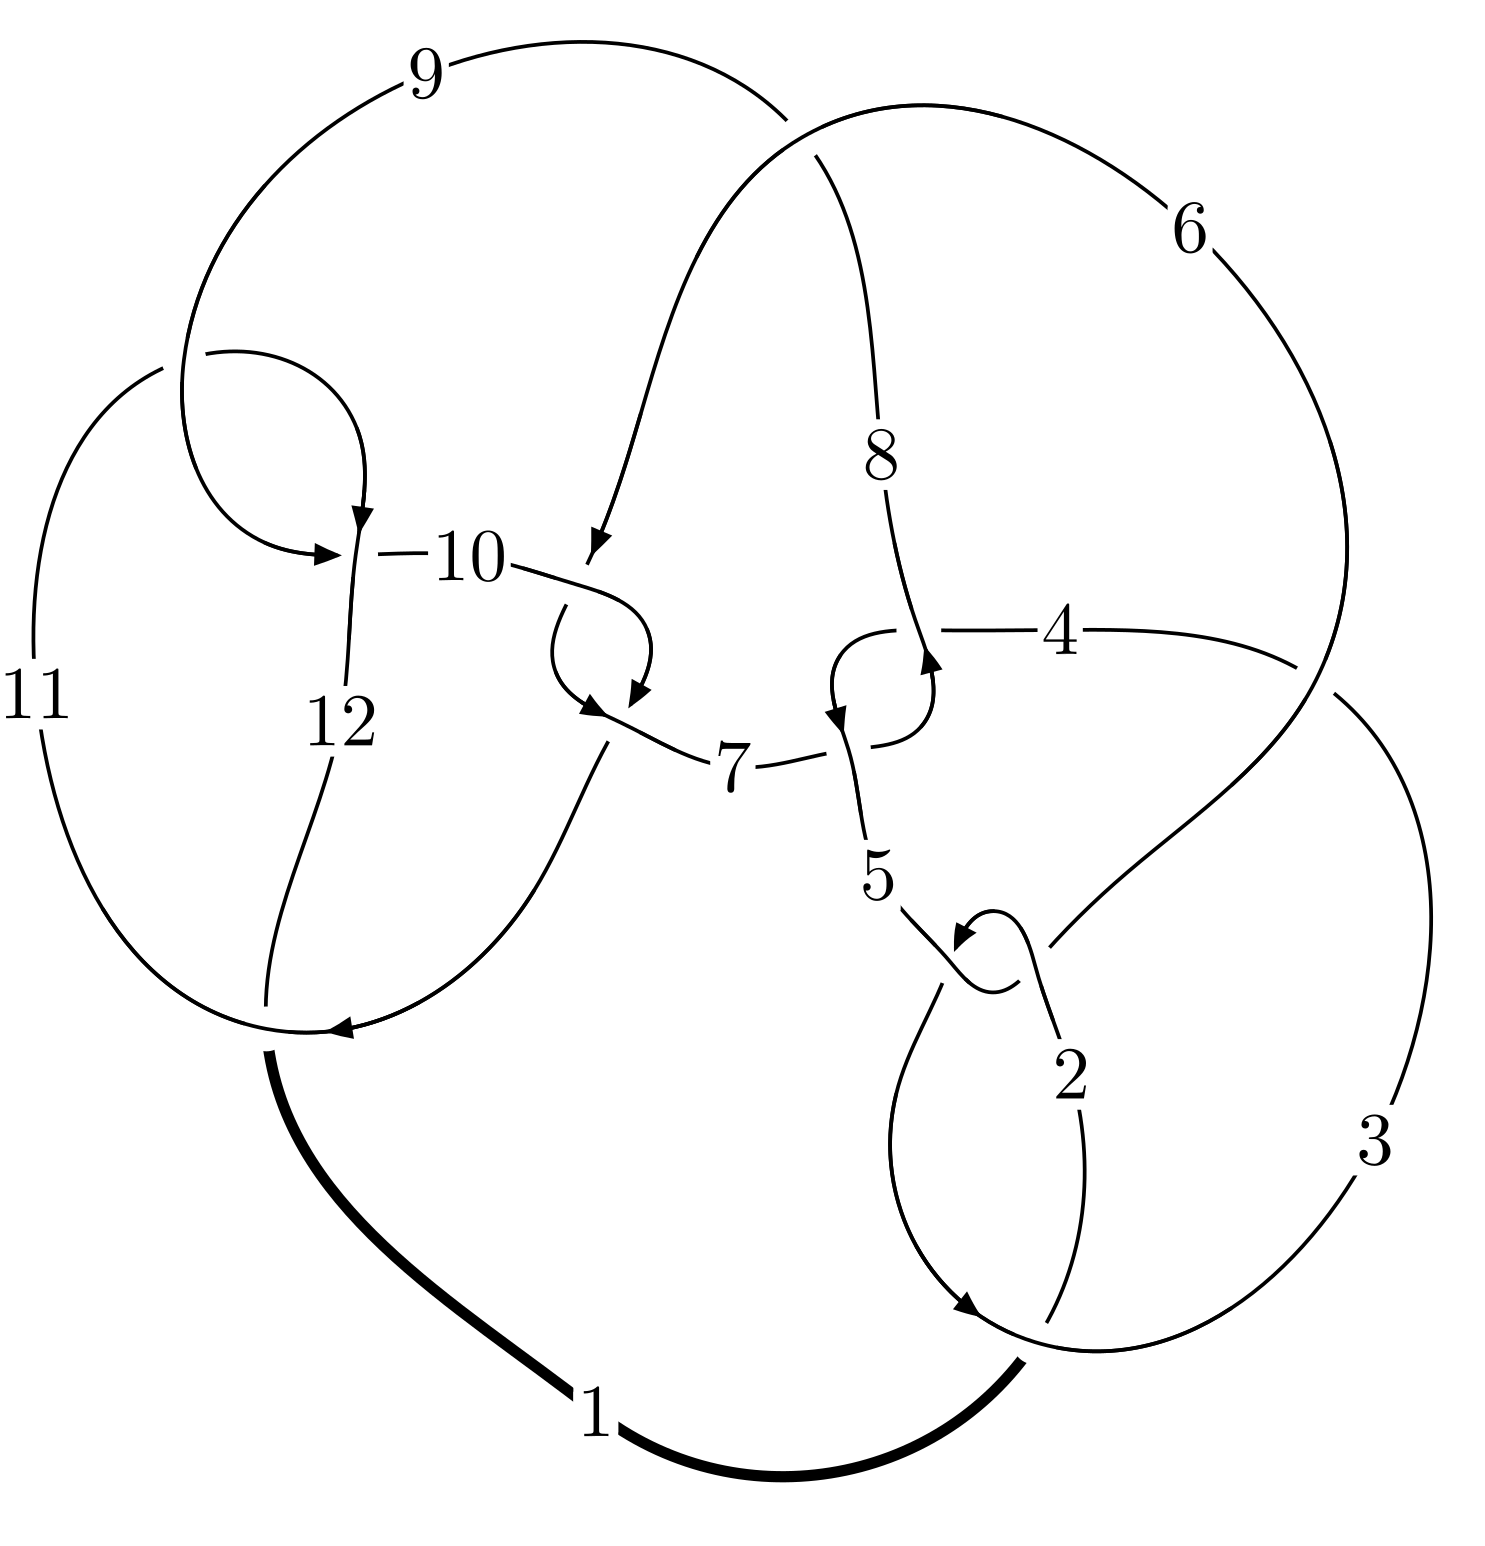
\includegraphics[width=112pt]{../../../GIT/diagram.site/Diagrams/png/2090_12n_0001.png}\\
\ \ \ A knot diagram\footnotemark}&
\allowdisplaybreaks
\textbf{Linearized knot diagam} \\
\cline{2-2}
 &
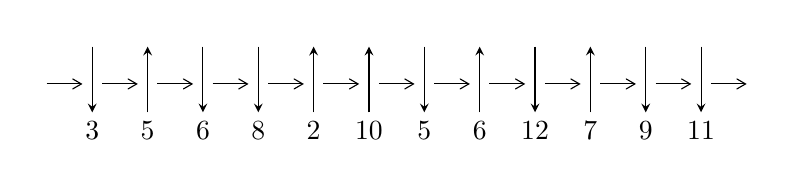
\begin{tikzpicture}[x=20pt, y=17pt]
	% nodes
	\node (C0) at (0, 0) {};
	\node (C1) at (1, 0) {};
	\node (C1U) at (1, +1) {};
	\node (C1D) at (1, -1) {3};

	\node (C2) at (2, 0) {};
	\node (C2U) at (2, +1) {};
	\node (C2D) at (2, -1) {5};

	\node (C3) at (3, 0) {};
	\node (C3U) at (3, +1) {};
	\node (C3D) at (3, -1) {6};

	\node (C4) at (4, 0) {};
	\node (C4U) at (4, +1) {};
	\node (C4D) at (4, -1) {8};

	\node (C5) at (5, 0) {};
	\node (C5U) at (5, +1) {};
	\node (C5D) at (5, -1) {2};

	\node (C6) at (6, 0) {};
	\node (C6U) at (6, +1) {};
	\node (C6D) at (6, -1) {10};

	\node (C7) at (7, 0) {};
	\node (C7U) at (7, +1) {};
	\node (C7D) at (7, -1) {5};

	\node (C8) at (8, 0) {};
	\node (C8U) at (8, +1) {};
	\node (C8D) at (8, -1) {6};

	\node (C9) at (9, 0) {};
	\node (C9U) at (9, +1) {};
	\node (C9D) at (9, -1) {12};

	\node (C10) at (10, 0) {};
	\node (C10U) at (10, +1) {};
	\node (C10D) at (10, -1) {7};

	\node (C11) at (11, 0) {};
	\node (C11U) at (11, +1) {};
	\node (C11D) at (11, -1) {9};

	\node (C12) at (12, 0) {};
	\node (C12U) at (12, +1) {};
	\node (C12D) at (12, -1) {11};
	\node (C13) at (13, 0) {};

	% arrows
	\draw[->,>={angle 60}]
	(C0) edge (C1) (C1) edge (C2) (C2) edge (C3) (C3) edge (C4) (C4) edge (C5) (C5) edge (C6) (C6) edge (C7) (C7) edge (C8) (C8) edge (C9) (C9) edge (C10) (C10) edge (C11) (C11) edge (C12) (C12) edge (C13) ;	\draw[->,>=stealth]
	(C1U) edge (C1D) (C2D) edge (C2U) (C3U) edge (C3D) (C4U) edge (C4D) (C5D) edge (C5U) (C6D) edge (C6U) (C7U) edge (C7D) (C8D) edge (C8U) (C9U) edge (C9D) (C10D) edge (C10U) (C11U) edge (C11D) (C12U) edge (C12D) ;
	\end{tikzpicture} \\
\hhline{~~} \\& 
\textbf{Solving Sequence} \\ \cline{2-2} 
 &
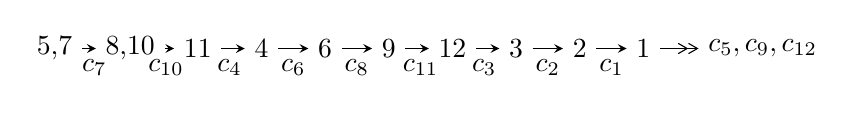
\begin{tikzpicture}[x=23pt, y=7pt]
	% node
	\node (A0) at (-1/8, 0) {5,7};
	\node (A1) at (17/16, 0) {8,10};
	\node (A2) at (17/8, 0) {11};
	\node (A3) at (25/8, 0) {4};
	\node (A4) at (33/8, 0) {6};
	\node (A5) at (41/8, 0) {9};
	\node (A6) at (49/8, 0) {12};
	\node (A7) at (57/8, 0) {3};
	\node (A8) at (65/8, 0) {2};
	\node (A9) at (73/8, 0) {1};
	\node (C1) at (1/2, -1) {$c_{7}$};
	\node (C2) at (13/8, -1) {$c_{10}$};
	\node (C3) at (21/8, -1) {$c_{4}$};
	\node (C4) at (29/8, -1) {$c_{6}$};
	\node (C5) at (37/8, -1) {$c_{8}$};
	\node (C6) at (45/8, -1) {$c_{11}$};
	\node (C7) at (53/8, -1) {$c_{3}$};
	\node (C8) at (61/8, -1) {$c_{2}$};
	\node (C9) at (69/8, -1) {$c_{1}$};
	\node (A10) at (11, 0) {$c_{5},c_{9},c_{12}$};

	% edge
	\draw[->,>=stealth]	
	(A0) edge (A1) (A1) edge (A2) (A2) edge (A3) (A3) edge (A4) (A4) edge (A5) (A5) edge (A6) (A6) edge (A7) (A7) edge (A8) (A8) edge (A9) ;
	\draw[->>,>={angle 60}]	
	(A9) edge (A10);
\end{tikzpicture} \\ 

\end{tabular} \\

\footnotetext{
The image of knot diagram is generated by the software ``\textbf{Draw programme}" developed by Andrew Bartholomew(\url{http://www.layer8.co.uk/maths/draw/index.htm\#Running-draw}), where we modified some parts for our purpose(\url{https://github.com/CATsTAILs/LinksPainter}).
}\phantom \\ \newline 
\centering \textbf{Ideals for irreducible components\footnotemark of $X_{\text{par}}$} 
 
\begin{align*}
I^u_{1}&=\langle 
4.37455\times10^{135} u^{43}-1.12079\times10^{136} u^{42}+\cdots+3.29429\times10^{139} b+3.17022\times10^{139},\\
\phantom{I^u_{1}}&\phantom{= \langle  }5.94999\times10^{134} u^{43}-5.65113\times10^{136} u^{42}+\cdots+1.31772\times10^{140} a-1.01004\times10^{141},\\
\phantom{I^u_{1}}&\phantom{= \langle  }u^{44}-2 u^{43}+\cdots+18432 u^2+4096\rangle \\
I^u_{2}&=\langle 
b,\;2 u^3+u^2+a+5 u+1,\;u^4+u^3+3 u^2+2 u+1\rangle \\
\\
I^v_{1}&=\langle 
a,\;-623 v^{11}+133 v^{10}+\cdots+263 b+608,\\
\phantom{I^v_{1}}&\phantom{= \langle  }v^{12}- v^{11}- v^{10}+6 v^9-5 v^8- v^7+5 v^6-9 v^5+11 v^4-7 v^3+4 v^2-3 v+1\rangle \\
\end{align*}
\raggedright * 3 irreducible components of $\dim_{\mathbb{C}}=0$, with total 60 representations.\\
\footnotetext{All coefficients of polynomials are rational numbers. But the coefficients are sometimes approximated in decimal forms when there is not enough margin.}
\newpage
\renewcommand{\arraystretch}{1}
\centering \section*{I. $I^u_{1}= \langle 4.37\times10^{135} u^{43}-1.12\times10^{136} u^{42}+\cdots+3.29\times10^{139} b+3.17\times10^{139},\;5.95\times10^{134} u^{43}-5.65\times10^{136} u^{42}+\cdots+1.32\times10^{140} a-1.01\times10^{141},\;u^{44}-2 u^{43}+\cdots+18432 u^2+4096 \rangle$}
\flushleft \textbf{(i) Arc colorings}\\
\begin{tabular}{m{7pt} m{180pt} m{7pt} m{180pt} }
\flushright $a_{5}=$&$\begin{pmatrix}0\\u\end{pmatrix}$ \\
\flushright $a_{7}=$&$\begin{pmatrix}1\\0\end{pmatrix}$ \\
\flushright $a_{8}=$&$\begin{pmatrix}1\\u^2\end{pmatrix}$ \\
\flushright $a_{10}=$&$\begin{pmatrix}-4.51538\times10^{-6} u^{43}+0.000428858 u^{42}+\cdots+11.6690 u+7.66506\\-0.000132792 u^{43}+0.000340222 u^{42}+\cdots-0.117088 u-0.962337\end{pmatrix}$ \\
\flushright $a_{11}=$&$\begin{pmatrix}-0.000137307 u^{43}+0.000769080 u^{42}+\cdots+11.5519 u+6.70273\\-0.000132792 u^{43}+0.000340222 u^{42}+\cdots-0.117088 u-0.962337\end{pmatrix}$ \\
\flushright $a_{4}=$&$\begin{pmatrix}u\\u^3+u\end{pmatrix}$ \\
\flushright $a_{6}=$&$\begin{pmatrix}0.0000465812 u^{43}-0.0000760961 u^{42}+\cdots-2.91296 u-1.00498\\-0.000146319 u^{43}+0.000385840 u^{42}+\cdots-0.577119 u-0.161513\end{pmatrix}$ \\
\flushright $a_{9}=$&$\begin{pmatrix}-0.0000233627 u^{43}+0.0000758354 u^{42}+\cdots+0.973632 u+0.112523\\-0.0000848623 u^{43}+0.000160319 u^{42}+\cdots+0.425724 u-0.685913\end{pmatrix}$ \\
\flushright $a_{12}=$&$\begin{pmatrix}-0.000153153 u^{43}+0.000767618 u^{42}+\cdots+10.5379 u+6.59579\\-0.0000848623 u^{43}+0.000160319 u^{42}+\cdots+0.425724 u-0.685913\end{pmatrix}$ \\
\flushright $a_{3}=$&$\begin{pmatrix}0.000294989 u^{43}-0.000566017 u^{42}+\cdots+5.23132 u+1.61723\\0.0000291099 u^{43}-0.0000723952 u^{42}+\cdots+0.112523 u+0.0956936\end{pmatrix}$ \\
\flushright $a_{2}=$&$\begin{pmatrix}0.000294989 u^{43}-0.000566017 u^{42}+\cdots+5.23132 u+1.61723\\0.0000637808 u^{43}-0.000165274 u^{42}+\cdots-1.09575 u-0.00245309\end{pmatrix}$ \\
\flushright $a_{1}=$&$\begin{pmatrix}-0.0000848166 u^{43}+0.000176172 u^{42}+\cdots+2.52664 u+0.913367\\-0.0000382354 u^{43}+0.000100076 u^{42}+\cdots-0.386322 u-0.0916094\end{pmatrix}$\\&\end{tabular}
\flushleft \textbf{(ii) Obstruction class $= -1$}\\~\\
\flushleft \textbf{(iii) Cusp Shapes $= 0.00275050 u^{43}-0.00388332 u^{42}+\cdots+65.4192 u+6.54832$}\\~\\
\newpage\renewcommand{\arraystretch}{1}
\flushleft \textbf{(iv) u-Polynomials at the component}\newline \\
\begin{tabular}{m{50pt}|m{274pt}}
Crossings & \hspace{64pt}u-Polynomials at each crossing \\
\hline $$\begin{aligned}c_{1}\end{aligned}$$&$\begin{aligned}
&u^{44}+8 u^{43}+\cdots+22 u+1
\end{aligned}$\\
\hline $$\begin{aligned}c_{2},c_{5}\end{aligned}$$&$\begin{aligned}
&u^{44}+8 u^{43}+\cdots+6 u+1
\end{aligned}$\\
\hline $$\begin{aligned}c_{3}\end{aligned}$$&$\begin{aligned}
&u^{44}-8 u^{43}+\cdots+577140 u+41508
\end{aligned}$\\
\hline $$\begin{aligned}c_{4},c_{7}\end{aligned}$$&$\begin{aligned}
&u^{44}-2 u^{43}+\cdots+18432 u^2+4096
\end{aligned}$\\
\hline $$\begin{aligned}c_{6},c_{10}\end{aligned}$$&$\begin{aligned}
&u^{44}-3 u^{43}+\cdots-120 u+16
\end{aligned}$\\
\hline $$\begin{aligned}c_{8}\end{aligned}$$&$\begin{aligned}
&u^{44}+4 u^{43}+\cdots+2 u+1
\end{aligned}$\\
\hline $$\begin{aligned}c_{9},c_{11}\end{aligned}$$&$\begin{aligned}
&u^{44}-7 u^{43}+\cdots+8 u+1
\end{aligned}$\\
\hline $$\begin{aligned}c_{12}\end{aligned}$$&$\begin{aligned}
&u^{44}+17 u^{43}+\cdots+48 u+1
\end{aligned}$\\
\hline
\end{tabular}\\~\\
\newpage\renewcommand{\arraystretch}{1}
\flushleft \textbf{(v) Riley Polynomials at the component}\newline \\
\begin{tabular}{m{50pt}|m{274pt}}
Crossings & \hspace{64pt}Riley Polynomials at each crossing \\
\hline $$\begin{aligned}c_{1}\end{aligned}$$&$\begin{aligned}
&y^{44}+64 y^{43}+\cdots+22 y+1
\end{aligned}$\\
\hline $$\begin{aligned}c_{2},c_{5}\end{aligned}$$&$\begin{aligned}
&y^{44}+8 y^{43}+\cdots+22 y+1
\end{aligned}$\\
\hline $$\begin{aligned}c_{3}\end{aligned}$$&$\begin{aligned}
&y^{44}+120 y^{43}+\cdots+42862402296 y+1722914064
\end{aligned}$\\
\hline $$\begin{aligned}c_{4},c_{7}\end{aligned}$$&$\begin{aligned}
&y^{44}+70 y^{43}+\cdots+150994944 y+16777216
\end{aligned}$\\
\hline $$\begin{aligned}c_{6},c_{10}\end{aligned}$$&$\begin{aligned}
&y^{44}-33 y^{43}+\cdots-576 y+256
\end{aligned}$\\
\hline $$\begin{aligned}c_{8}\end{aligned}$$&$\begin{aligned}
&y^{44}-80 y^{43}+\cdots+14 y+1
\end{aligned}$\\
\hline $$\begin{aligned}c_{9},c_{11}\end{aligned}$$&$\begin{aligned}
&y^{44}-17 y^{43}+\cdots-48 y+1
\end{aligned}$\\
\hline $$\begin{aligned}c_{12}\end{aligned}$$&$\begin{aligned}
&y^{44}+27 y^{43}+\cdots-48 y+1
\end{aligned}$\\
\hline
\end{tabular}\\~\\
\newpage\flushleft \textbf{(vi) Complex Volumes and Cusp Shapes}
$$\begin{array}{c|c|c}  
\text{Solutions to }I^u_{1}& \I (\text{vol} + \sqrt{-1}CS) & \text{Cusp shape}\\
 \hline 
\begin{aligned}
u &= -0.587750 + 0.727199 I \\
a &= \phantom{-}0.306966 - 0.640744 I \\
b &= -1.002580 + 0.067245 I\end{aligned}
 & \phantom{-}0.0012605 + 0.0509035 I & -2.15533 + 0.17848 I \\ \hline\begin{aligned}
u &= -0.587750 - 0.727199 I \\
a &= \phantom{-}0.306966 + 0.640744 I \\
b &= -1.002580 - 0.067245 I\end{aligned}
 & \phantom{-}0.0012605 - 0.0509035 I & -2.15533 - 0.17848 I \\ \hline\begin{aligned}
u &= \phantom{-}0.730847 + 0.390041 I \\
a &= \phantom{-}0.437616 - 0.402493 I \\
b &= -1.132220 - 0.401644 I\end{aligned}
 & \phantom{-}2.44756 + 1.58887 I & \phantom{-}2.11619 + 0.16814 I \\ \hline\begin{aligned}
u &= \phantom{-}0.730847 - 0.390041 I \\
a &= \phantom{-}0.437616 + 0.402493 I \\
b &= -1.132220 + 0.401644 I\end{aligned}
 & \phantom{-}2.44756 - 1.58887 I & \phantom{-}2.11619 - 0.16814 I \\ \hline\begin{aligned}
u &= -0.611739 + 0.487067 I \\
a &= -0.156519 + 0.760305 I \\
b &= \phantom{-}1.033990 + 0.442395 I\end{aligned}
 & -0.96246 + 4.43252 I & -5.23001 - 6.92056 I \\ \hline\begin{aligned}
u &= -0.611739 - 0.487067 I \\
a &= -0.156519 - 0.760305 I \\
b &= \phantom{-}1.033990 - 0.442395 I\end{aligned}
 & -0.96246 - 4.43252 I & -5.23001 + 6.92056 I \\ \hline\begin{aligned}
u &= -0.496705 + 0.586520 I \\
a &= \phantom{-}0.803429 - 0.614772 I \\
b &= -0.139559 - 0.567313 I\end{aligned}
 & \phantom{-}0.003759 + 1.358260 I & \phantom{-}0.43877 - 4.70156 I \\ \hline\begin{aligned}
u &= -0.496705 - 0.586520 I \\
a &= \phantom{-}0.803429 + 0.614772 I \\
b &= -0.139559 + 0.567313 I\end{aligned}
 & \phantom{-}0.003759 - 1.358260 I & \phantom{-}0.43877 + 4.70156 I \\ \hline\begin{aligned}
u &= \phantom{-}0.579885 + 0.494350 I \\
a &= -0.225969 + 0.616510 I \\
b &= \phantom{-}1.124200 + 0.621018 I\end{aligned}
 & \phantom{-}0.29937 + 6.78003 I & -1.02805 - 2.83496 I \\ \hline\begin{aligned}
u &= \phantom{-}0.579885 - 0.494350 I \\
a &= -0.225969 - 0.616510 I \\
b &= \phantom{-}1.124200 - 0.621018 I\end{aligned}
 & \phantom{-}0.29937 - 6.78003 I & -1.02805 + 2.83496 I\\
 \hline 
 \end{array}$$\newpage$$\begin{array}{c|c|c}  
\text{Solutions to }I^u_{1}& \I (\text{vol} + \sqrt{-1}CS) & \text{Cusp shape}\\
 \hline 
\begin{aligned}
u &= -0.511627 + 0.444892 I \\
a &= \phantom{-}1.093280 - 0.445499 I \\
b &= \phantom{-}0.072410 - 0.459091 I\end{aligned}
 & -0.021919 + 1.380100 I & -0.83838 - 4.05172 I \\ \hline\begin{aligned}
u &= -0.511627 - 0.444892 I \\
a &= \phantom{-}1.093280 + 0.445499 I \\
b &= \phantom{-}0.072410 + 0.459091 I\end{aligned}
 & -0.021919 - 1.380100 I & -0.83838 + 4.05172 I \\ \hline\begin{aligned}
u &= \phantom{-}0.299193 + 0.591308 I \\
a &= \phantom{-}2.27653 - 0.10382 I \\
b &= -0.095849 + 0.693490 I\end{aligned}
 & -1.10964 + 2.86683 I & -0.194269 - 1.150607 I \\ \hline\begin{aligned}
u &= \phantom{-}0.299193 - 0.591308 I \\
a &= \phantom{-}2.27653 + 0.10382 I \\
b &= -0.095849 - 0.693490 I\end{aligned}
 & -1.10964 - 2.86683 I & -0.194269 + 1.150607 I \\ \hline\begin{aligned}
u &= -0.524212 + 0.325358 I \\
a &= -0.254256 + 1.159040 I \\
b &= \phantom{-}0.408649 + 0.820268 I\end{aligned}
 & -1.87563 - 1.38329 I & -4.88472 + 0.88974 I \\ \hline\begin{aligned}
u &= -0.524212 - 0.325358 I \\
a &= -0.254256 - 1.159040 I \\
b &= \phantom{-}0.408649 - 0.820268 I\end{aligned}
 & -1.87563 + 1.38329 I & -4.88472 - 0.88974 I \\ \hline\begin{aligned}
u &= \phantom{-}0.418662 + 0.429381 I \\
a &= -1.12716 + 1.24862 I \\
b &= \phantom{-}0.573000 + 0.460129 I\end{aligned}
 & -2.37055 - 0.63845 I & -5.51576 - 1.51985 I \\ \hline\begin{aligned}
u &= \phantom{-}0.418662 - 0.429381 I \\
a &= -1.12716 - 1.24862 I \\
b &= \phantom{-}0.573000 - 0.460129 I\end{aligned}
 & -2.37055 + 0.63845 I & -5.51576 + 1.51985 I \\ \hline\begin{aligned}
u &= -0.89693 + 1.10743 I \\
a &= -0.995115 + 0.841611 I \\
b &= \phantom{-}1.367840 + 0.047642 I\end{aligned}
 & \phantom{-}3.71063 - 1.12943 I & \phantom{-0.000000 } 0 \\ \hline\begin{aligned}
u &= -0.89693 - 1.10743 I \\
a &= -0.995115 - 0.841611 I \\
b &= \phantom{-}1.367840 - 0.047642 I\end{aligned}
 & \phantom{-}3.71063 + 1.12943 I & \phantom{-0.000000 } 0\\
 \hline 
 \end{array}$$\newpage$$\begin{array}{c|c|c}  
\text{Solutions to }I^u_{1}& \I (\text{vol} + \sqrt{-1}CS) & \text{Cusp shape}\\
 \hline 
\begin{aligned}
u &= -0.11702 + 1.45676 I \\
a &= -0.0541211 - 0.0270150 I \\
b &= -0.525995 + 0.033075 I\end{aligned}
 & \phantom{-}5.55211 + 3.08791 I & \phantom{-0.000000 } 0 \\ \hline\begin{aligned}
u &= -0.11702 - 1.45676 I \\
a &= -0.0541211 + 0.0270150 I \\
b &= -0.525995 - 0.033075 I\end{aligned}
 & \phantom{-}5.55211 - 3.08791 I & \phantom{-0.000000 } 0 \\ \hline\begin{aligned}
u &= -0.50581 + 1.37651 I \\
a &= \phantom{-}1.240180 - 0.406596 I \\
b &= -1.36837 + 0.37289 I\end{aligned}
 & \phantom{-}3.06981 - 7.05974 I & \phantom{-0.000000 } 0 \\ \hline\begin{aligned}
u &= -0.50581 - 1.37651 I \\
a &= \phantom{-}1.240180 + 0.406596 I \\
b &= -1.36837 - 0.37289 I\end{aligned}
 & \phantom{-}3.06981 + 7.05974 I & \phantom{-0.000000 } 0 \\ \hline\begin{aligned}
u &= \phantom{-}0.175618 + 0.424295 I \\
a &= \phantom{-}6.42637 + 3.07840 I \\
b &= -0.342417 + 0.239754 I\end{aligned}
 & -1.92351 - 1.76678 I & \phantom{-}8.1243 + 28.0957 I \\ \hline\begin{aligned}
u &= \phantom{-}0.175618 - 0.424295 I \\
a &= \phantom{-}6.42637 - 3.07840 I \\
b &= -0.342417 - 0.239754 I\end{aligned}
 & -1.92351 + 1.76678 I & \phantom{-}8.1243 - 28.0957 I \\ \hline\begin{aligned}
u &= \phantom{-}1.11832 + 1.28481 I \\
a &= \phantom{-}0.800873 + 0.371072 I \\
b &= -1.46830 - 0.16447 I\end{aligned}
 & \phantom{-}5.66847 + 1.40169 I & \phantom{-0.000000 } 0 \\ \hline\begin{aligned}
u &= \phantom{-}1.11832 - 1.28481 I \\
a &= \phantom{-}0.800873 - 0.371072 I \\
b &= -1.46830 + 0.16447 I\end{aligned}
 & \phantom{-}5.66847 - 1.40169 I & \phantom{-0.000000 } 0 \\ \hline\begin{aligned}
u &= \phantom{-}1.44144 + 0.90992 I \\
a &= -0.651114 - 0.640799 I \\
b &= \phantom{-}1.46122 - 0.25816 I\end{aligned}
 & \phantom{-}5.49304 - 4.87559 I & \phantom{-0.000000 } 0 \\ \hline\begin{aligned}
u &= \phantom{-}1.44144 - 0.90992 I \\
a &= -0.651114 + 0.640799 I \\
b &= \phantom{-}1.46122 + 0.25816 I\end{aligned}
 & \phantom{-}5.49304 + 4.87559 I & \phantom{-0.000000 } 0\\
 \hline 
 \end{array}$$\newpage$$\begin{array}{c|c|c}  
\text{Solutions to }I^u_{1}& \I (\text{vol} + \sqrt{-1}CS) & \text{Cusp shape}\\
 \hline 
\begin{aligned}
u &= \phantom{-}0.19127 + 2.08900 I \\
a &= \phantom{-}1.45451 + 0.12813 I \\
b &= -1.301920 + 0.064317 I\end{aligned}
 & \phantom{-}8.56289 - 3.55763 I & \phantom{-0.000000 } 0 \\ \hline\begin{aligned}
u &= \phantom{-}0.19127 - 2.08900 I \\
a &= \phantom{-}1.45451 - 0.12813 I \\
b &= -1.301920 - 0.064317 I\end{aligned}
 & \phantom{-}8.56289 + 3.55763 I & \phantom{-0.000000 } 0 \\ \hline\begin{aligned}
u &= -0.36840 + 2.10955 I \\
a &= -0.0581272 + 0.0787356 I \\
b &= -0.280354 + 1.371580 I\end{aligned}
 & \phantom{-}10.23040 + 6.56728 I & \phantom{-0.000000 } 0 \\ \hline\begin{aligned}
u &= -0.36840 - 2.10955 I \\
a &= -0.0581272 - 0.0787356 I \\
b &= -0.280354 - 1.371580 I\end{aligned}
 & \phantom{-}10.23040 - 6.56728 I & \phantom{-0.000000 } 0 \\ \hline\begin{aligned}
u &= \phantom{-}0.76685 + 2.01630 I \\
a &= \phantom{-}1.004910 + 0.650911 I \\
b &= -1.42673 + 0.75889 I\end{aligned}
 & \phantom{-}13.8428 - 14.0825 I & \phantom{-0.000000 } 0 \\ \hline\begin{aligned}
u &= \phantom{-}0.76685 - 2.01630 I \\
a &= \phantom{-}1.004910 - 0.650911 I \\
b &= -1.42673 - 0.75889 I\end{aligned}
 & \phantom{-}13.8428 + 14.0825 I & \phantom{-0.000000 } 0 \\ \hline\begin{aligned}
u &= -0.01900 + 2.17067 I \\
a &= \phantom{-}0.0496534 - 0.0826517 I \\
b &= -0.160771 - 1.385870 I\end{aligned}
 & \phantom{-}10.46560 + 0.62164 I & \phantom{-0.000000 } 0 \\ \hline\begin{aligned}
u &= -0.01900 - 2.17067 I \\
a &= \phantom{-}0.0496534 + 0.0826517 I \\
b &= -0.160771 + 1.385870 I\end{aligned}
 & \phantom{-}10.46560 - 0.62164 I & \phantom{-0.000000 } 0 \\ \hline\begin{aligned}
u &= \phantom{-}0.61800 + 2.21033 I \\
a &= -1.060520 - 0.447387 I \\
b &= \phantom{-}1.56771 - 0.52759 I\end{aligned}
 & \phantom{-}16.1314 - 7.4218 I & \phantom{-0.000000 } 0 \\ \hline\begin{aligned}
u &= \phantom{-}0.61800 - 2.21033 I \\
a &= -1.060520 + 0.447387 I \\
b &= \phantom{-}1.56771 + 0.52759 I\end{aligned}
 & \phantom{-}16.1314 + 7.4218 I & \phantom{-0.000000 } 0\\
 \hline 
 \end{array}$$\newpage$$\begin{array}{c|c|c}  
\text{Solutions to }I^u_{1}& \I (\text{vol} + \sqrt{-1}CS) & \text{Cusp shape}\\
 \hline 
\begin{aligned}
u &= -0.48180 + 2.24551 I \\
a &= \phantom{-}0.994426 - 0.463135 I \\
b &= -1.49947 - 0.71295 I\end{aligned}
 & \phantom{-}14.6778 + 6.8524 I & \phantom{-0.000000 } 0 \\ \hline\begin{aligned}
u &= -0.48180 - 2.24551 I \\
a &= \phantom{-}0.994426 + 0.463135 I \\
b &= -1.49947 + 0.71295 I\end{aligned}
 & \phantom{-}14.6778 - 6.8524 I & \phantom{-0.000000 } 0 \\ \hline\begin{aligned}
u &= -0.21908 + 2.39343 I \\
a &= -1.055840 + 0.248840 I \\
b &= \phantom{-}1.63553 + 0.43161 I\end{aligned}
 & \phantom{-}16.6724 + 0.0015 I & \phantom{-0.000000 } 0 \\ \hline\begin{aligned}
u &= -0.21908 - 2.39343 I \\
a &= -1.055840 - 0.248840 I \\
b &= \phantom{-}1.63553 - 0.43161 I\end{aligned}
 & \phantom{-}16.6724 - 0.0015 I & \phantom{-0.000000 } 0\\
 \hline 
 \end{array}$$\newpage\newpage\renewcommand{\arraystretch}{1}
\centering \section*{II. $I^u_{2}= \langle b,\;2 u^3+u^2+a+5 u+1,\;u^4+u^3+3 u^2+2 u+1 \rangle$}
\flushleft \textbf{(i) Arc colorings}\\
\begin{tabular}{m{7pt} m{180pt} m{7pt} m{180pt} }
\flushright $a_{5}=$&$\begin{pmatrix}0\\u\end{pmatrix}$ \\
\flushright $a_{7}=$&$\begin{pmatrix}1\\0\end{pmatrix}$ \\
\flushright $a_{8}=$&$\begin{pmatrix}1\\u^2\end{pmatrix}$ \\
\flushright $a_{10}=$&$\begin{pmatrix}-2 u^3- u^2-5 u-1\\0\end{pmatrix}$ \\
\flushright $a_{11}=$&$\begin{pmatrix}-2 u^3- u^2-5 u-1\\0\end{pmatrix}$ \\
\flushright $a_{4}=$&$\begin{pmatrix}u\\u^3+u\end{pmatrix}$ \\
\flushright $a_{6}=$&$\begin{pmatrix}1\\0\end{pmatrix}$ \\
\flushright $a_{9}=$&$\begin{pmatrix}u^2+1\\u^2\end{pmatrix}$ \\
\flushright $a_{12}=$&$\begin{pmatrix}-2 u^3-2 u^2-5 u-2\\- u^2\end{pmatrix}$ \\
\flushright $a_{3}=$&$\begin{pmatrix}u^3+2 u\\u^3+u\end{pmatrix}$ \\
\flushright $a_{2}=$&$\begin{pmatrix}u^3+2 u\\u^3+u^2+2 u+1\end{pmatrix}$ \\
\flushright $a_{1}=$&$\begin{pmatrix}- u^2-1\\- u^2\end{pmatrix}$\\&\end{tabular}
\flushleft \textbf{(ii) Obstruction class $= 1$}\\~\\
\flushleft \textbf{(iii) Cusp Shapes $= 3 u^2-2 u-1$}\\~\\
\newpage\renewcommand{\arraystretch}{1}
\flushleft \textbf{(iv) u-Polynomials at the component}\newline \\
\begin{tabular}{m{50pt}|m{274pt}}
Crossings & \hspace{64pt}u-Polynomials at each crossing \\
\hline $$\begin{aligned}c_{1},c_{4}\end{aligned}$$&$\begin{aligned}
&u^4- u^3+3 u^2-2 u+1
\end{aligned}$\\
\hline $$\begin{aligned}c_{2}\end{aligned}$$&$\begin{aligned}
&u^4- u^3+u^2+1
\end{aligned}$\\
\hline $$\begin{aligned}c_{3}\end{aligned}$$&$\begin{aligned}
&u^4+u^3+5 u^2- u+2
\end{aligned}$\\
\hline $$\begin{aligned}c_{5}\end{aligned}$$&$\begin{aligned}
&u^4+u^3+u^2+1
\end{aligned}$\\
\hline $$\begin{aligned}c_{6},c_{10}\end{aligned}$$&$\begin{aligned}
&u^4
\end{aligned}$\\
\hline $$\begin{aligned}c_{7}\end{aligned}$$&$\begin{aligned}
&u^4+u^3+3 u^2+2 u+1
\end{aligned}$\\
\hline $$\begin{aligned}c_{8}\end{aligned}$$&$\begin{aligned}
&u^4-5 u^3+7 u^2-2 u+1
\end{aligned}$\\
\hline $$\begin{aligned}c_{9}\end{aligned}$$&$\begin{aligned}
&(u-1)^4
\end{aligned}$\\
\hline $$\begin{aligned}c_{11},c_{12}\end{aligned}$$&$\begin{aligned}
&(u+1)^4
\end{aligned}$\\
\hline
\end{tabular}\\~\\
\newpage\renewcommand{\arraystretch}{1}
\flushleft \textbf{(v) Riley Polynomials at the component}\newline \\
\begin{tabular}{m{50pt}|m{274pt}}
Crossings & \hspace{64pt}Riley Polynomials at each crossing \\
\hline $$\begin{aligned}c_{1},c_{4},c_{7}\end{aligned}$$&$\begin{aligned}
&y^4+5 y^3+7 y^2+2 y+1
\end{aligned}$\\
\hline $$\begin{aligned}c_{2},c_{5}\end{aligned}$$&$\begin{aligned}
&y^4+y^3+3 y^2+2 y+1
\end{aligned}$\\
\hline $$\begin{aligned}c_{3}\end{aligned}$$&$\begin{aligned}
&y^4+9 y^3+31 y^2+19 y+4
\end{aligned}$\\
\hline $$\begin{aligned}c_{6},c_{10}\end{aligned}$$&$\begin{aligned}
&y^4
\end{aligned}$\\
\hline $$\begin{aligned}c_{8}\end{aligned}$$&$\begin{aligned}
&y^4-11 y^3+31 y^2+10 y+1
\end{aligned}$\\
\hline $$\begin{aligned}c_{9},c_{11},c_{12}\end{aligned}$$&$\begin{aligned}
&(y-1)^4
\end{aligned}$\\
\hline
\end{tabular}\\~\\
\newpage\flushleft \textbf{(vi) Complex Volumes and Cusp Shapes}
$$\begin{array}{c|c|c}  
\text{Solutions to }I^u_{2}& \I (\text{vol} + \sqrt{-1}CS) & \text{Cusp shape}\\
 \hline 
\begin{aligned}
u &= -0.395123 + 0.506844 I \\
a &= \phantom{-}0.59074 - 2.34806 I \\
b &= \phantom{-0.000000 } 0\end{aligned}
 & -1.85594 + 1.41510 I & -0.51206 - 2.21528 I \\ \hline\begin{aligned}
u &= -0.395123 - 0.506844 I \\
a &= \phantom{-}0.59074 + 2.34806 I \\
b &= \phantom{-0.000000 } 0\end{aligned}
 & -1.85594 - 1.41510 I & -0.51206 + 2.21528 I \\ \hline\begin{aligned}
u &= -0.10488 + 1.55249 I \\
a &= \phantom{-}0.409261 - 0.055548 I \\
b &= \phantom{-0.000000 } 0\end{aligned}
 & \phantom{-}5.14581 + 3.16396 I & -7.98794 - 4.08190 I \\ \hline\begin{aligned}
u &= -0.10488 - 1.55249 I \\
a &= \phantom{-}0.409261 + 0.055548 I \\
b &= \phantom{-0.000000 } 0\end{aligned}
 & \phantom{-}5.14581 - 3.16396 I & -7.98794 + 4.08190 I\\
 \hline 
 \end{array}$$\newpage\newpage\renewcommand{\arraystretch}{1}
\centering \section*{III. $I^v_{1}= \langle a,\;-623 v^{11}+133 v^{10}+\cdots+263 b+608,\;v^{12}- v^{11}+\cdots-3 v+1 \rangle$}
\flushleft \textbf{(i) Arc colorings}\\
\begin{tabular}{m{7pt} m{180pt} m{7pt} m{180pt} }
\flushright $a_{5}=$&$\begin{pmatrix}v\\0\end{pmatrix}$ \\
\flushright $a_{7}=$&$\begin{pmatrix}1\\0\end{pmatrix}$ \\
\flushright $a_{8}=$&$\begin{pmatrix}1\\0\end{pmatrix}$ \\
\flushright $a_{10}=$&$\begin{pmatrix}0\\2.36882 v^{11}-0.505703 v^{10}+\cdots+5.05323 v-2.31179\end{pmatrix}$ \\
\flushright $a_{11}=$&$\begin{pmatrix}2.36882 v^{11}-0.505703 v^{10}+\cdots+5.05323 v-2.31179\\2.36882 v^{11}-0.505703 v^{10}+\cdots+5.05323 v-2.31179\end{pmatrix}$ \\
\flushright $a_{4}=$&$\begin{pmatrix}v\\0\end{pmatrix}$ \\
\flushright $a_{6}=$&$\begin{pmatrix}1\\6.30038 v^{11}-2.03042 v^{10}+\cdots+12.9506 v-7.99620\end{pmatrix}$ \\
\flushright $a_{9}=$&$\begin{pmatrix}-6.30038 v^{11}+2.03042 v^{10}+\cdots-12.9506 v+8.99620\\-10.9962 v^{11}+3.69582 v^{10}+\cdots-22.4943 v+16.0380\end{pmatrix}$ \\
\flushright $a_{12}=$&$\begin{pmatrix}-4.69582 v^{11}+1.66540 v^{10}+\cdots-9.54373 v+7.04183\\-10.9962 v^{11}+3.69582 v^{10}+\cdots-22.4943 v+16.0380\end{pmatrix}$ \\
\flushright $a_{3}=$&$\begin{pmatrix}-4.26996 v^{11}+1.59696 v^{10}+\cdots-9.90494 v+6.30038\\-7.30038 v^{11}+3.03042 v^{10}+\cdots-16.9506 v+10.9962\end{pmatrix}$ \\
\flushright $a_{2}=$&$\begin{pmatrix}-1.59696 v^{11}+0.756654 v^{10}+\cdots-4.39544 v+2.03042\\-7.30038 v^{11}+3.03042 v^{10}+\cdots-16.9506 v+10.9962\end{pmatrix}$ \\
\flushright $a_{1}=$&$\begin{pmatrix}-1\\-6.30038 v^{11}+2.03042 v^{10}+\cdots-12.9506 v+7.99620\end{pmatrix}$\\&\end{tabular}
\flushleft \textbf{(ii) Obstruction class $= 1$}\\~\\
\flushleft \textbf{(iii) Cusp Shapes $= -\frac{3729}{263} v^{11}+\frac{1130}{263} v^{10}+\frac{4668}{263} v^9-\frac{19527}{263} v^8+\frac{5107}{263} v^7+\frac{8452}{263} v^6-\frac{14914}{263} v^5+\frac{24322}{263} v^4-\frac{22832}{263} v^3+\frac{7241}{263} v^2-\frac{5199}{263} v+\frac{4001}{263}$}\\~\\
\newpage\renewcommand{\arraystretch}{1}
\flushleft \textbf{(iv) u-Polynomials at the component}\newline \\
\begin{tabular}{m{50pt}|m{274pt}}
Crossings & \hspace{64pt}u-Polynomials at each crossing \\
\hline $$\begin{aligned}c_{1},c_{3},c_{5}\end{aligned}$$&$\begin{aligned}
&(u^2- u+1)^6
\end{aligned}$\\
\hline $$\begin{aligned}c_{2}\end{aligned}$$&$\begin{aligned}
&(u^2+u+1)^6
\end{aligned}$\\
\hline $$\begin{aligned}c_{4},c_{7}\end{aligned}$$&$\begin{aligned}
&u^{12}
\end{aligned}$\\
\hline $$\begin{aligned}c_{6},c_{11}\end{aligned}$$&$\begin{aligned}
&(u^6- u^5- u^4+2 u^3- u+1)^2
\end{aligned}$\\
\hline $$\begin{aligned}c_{8}\end{aligned}$$&$\begin{aligned}
&(u^6-3 u^5+5 u^4-4 u^3+2 u^2- u+1)^2
\end{aligned}$\\
\hline $$\begin{aligned}c_{9},c_{10}\end{aligned}$$&$\begin{aligned}
&(u^6+u^5- u^4-2 u^3+u+1)^2
\end{aligned}$\\
\hline $$\begin{aligned}c_{12}\end{aligned}$$&$\begin{aligned}
&(u^6+3 u^5+5 u^4+4 u^3+2 u^2+u+1)^2
\end{aligned}$\\
\hline
\end{tabular}\\~\\
\newpage\renewcommand{\arraystretch}{1}
\flushleft \textbf{(v) Riley Polynomials at the component}\newline \\
\begin{tabular}{m{50pt}|m{274pt}}
Crossings & \hspace{64pt}Riley Polynomials at each crossing \\
\hline $$\begin{aligned}c_{1},c_{2},c_{3}\\c_{5}\end{aligned}$$&$\begin{aligned}
&(y^2+y+1)^6
\end{aligned}$\\
\hline $$\begin{aligned}c_{4},c_{7}\end{aligned}$$&$\begin{aligned}
&y^{12}
\end{aligned}$\\
\hline $$\begin{aligned}c_{6},c_{9},c_{10}\\c_{11}\end{aligned}$$&$\begin{aligned}
&(y^6-3 y^5+5 y^4-4 y^3+2 y^2- y+1)^2
\end{aligned}$\\
\hline $$\begin{aligned}c_{8},c_{12}\end{aligned}$$&$\begin{aligned}
&(y^6+y^5+5 y^4+6 y^2+3 y+1)^2
\end{aligned}$\\
\hline
\end{tabular}\\~\\
\newpage\flushleft \textbf{(vi) Complex Volumes and Cusp Shapes}
$$\begin{array}{c|c|c}  
\text{Solutions to }I^v_{1}& \I (\text{vol} + \sqrt{-1}CS) & \text{Cusp shape}\\
 \hline 
\begin{aligned}
v &= \phantom{-}0.815127 + 0.417821 I \\
a &= \phantom{-0.000000 } 0 \\
b &= -1.002190 - 0.295542 I\end{aligned}
 & \phantom{-}1.89061 - 1.10558 I & \phantom{-}2.90246 + 2.38339 I \\ \hline\begin{aligned}
v &= \phantom{-}0.815127 - 0.417821 I \\
a &= \phantom{-0.000000 } 0 \\
b &= -1.002190 + 0.295542 I\end{aligned}
 & \phantom{-}1.89061 + 1.10558 I & \phantom{-}2.90246 - 2.38339 I \\ \hline\begin{aligned}
v &= -0.045720 + 0.914831 I \\
a &= \phantom{-0.000000 } 0 \\
b &= -1.002190 + 0.295542 I\end{aligned}
 & \phantom{-}1.89061 - 2.95419 I & -0.30406 + 4.29351 I \\ \hline\begin{aligned}
v &= -0.045720 - 0.914831 I \\
a &= \phantom{-0.000000 } 0 \\
b &= -1.002190 - 0.295542 I\end{aligned}
 & \phantom{-}1.89061 + 2.95419 I & -0.30406 - 4.29351 I \\ \hline\begin{aligned}
v &= \phantom{-}0.679704 + 0.059778 I \\
a &= \phantom{-0.000000 } 0 \\
b &= \phantom{-}1.073950 + 0.558752 I\end{aligned}
 & \phantom{-0.000000 -}3.66314 I & \phantom{-}0.57335 - 2.34011 I \\ \hline\begin{aligned}
v &= \phantom{-}0.679704 - 0.059778 I \\
a &= \phantom{-0.000000 } 0 \\
b &= \phantom{-}1.073950 - 0.558752 I\end{aligned}
 & \phantom{-0.000000 } -3.66314 I & \phantom{-}0.57335 + 2.34011 I \\ \hline\begin{aligned}
v &= -0.288082 + 0.618530 I \\
a &= \phantom{-0.000000 } 0 \\
b &= \phantom{-}1.073950 - 0.558752 I\end{aligned}
 & \phantom{-0.000000 } -7.72290 I & -3.68173 + 10.26242 I \\ \hline\begin{aligned}
v &= -0.288082 - 0.618530 I \\
a &= \phantom{-0.000000 } 0 \\
b &= \phantom{-}1.073950 + 0.558752 I\end{aligned}
 & \phantom{-0.000000 -}7.72290 I & -3.68173 - 10.26242 I \\ \hline\begin{aligned}
v &= \phantom{-}0.93136 + 1.30101 I \\
a &= \phantom{-0.000000 } 0 \\
b &= \phantom{-}0.428243 - 0.664531 I\end{aligned}
 & -1.89061 + 2.95419 I & -6.66783 - 2.20469 I \\ \hline\begin{aligned}
v &= \phantom{-}0.93136 - 1.30101 I \\
a &= \phantom{-0.000000 } 0 \\
b &= \phantom{-}0.428243 + 0.664531 I\end{aligned}
 & -1.89061 - 2.95419 I & -6.66783 + 2.20469 I\\
 \hline 
 \end{array}$$\newpage$$\begin{array}{c|c|c}  
\text{Solutions to }I^v_{1}& \I (\text{vol} + \sqrt{-1}CS) & \text{Cusp shape}\\
 \hline 
\begin{aligned}
v &= -1.59239 + 0.15607 I \\
a &= \phantom{-0.000000 } 0 \\
b &= \phantom{-}0.428243 - 0.664531 I\end{aligned}
 & -1.89061 - 1.10558 I & -2.82220 + 2.24866 I \\ \hline\begin{aligned}
v &= -1.59239 - 0.15607 I \\
a &= \phantom{-0.000000 } 0 \\
b &= \phantom{-}0.428243 + 0.664531 I\end{aligned}
 & -1.89061 + 1.10558 I & -2.82220 - 2.24866 I\\
 \hline 
 \end{array}$$\newpage
\newpage\renewcommand{\arraystretch}{1}
\centering \section*{ IV. u-Polynomials}
\begin{tabular}{m{50pt}|m{274pt}}
Crossings & \hspace{64pt}u-Polynomials at each crossing \\
\hline $$\begin{aligned}c_{1}\end{aligned}$$&$\begin{aligned}
&((u^2- u+1)^6)(u^4- u^3+3 u^2-2 u+1)(u^{44}+8 u^{43}+\cdots+22 u+1)
\end{aligned}$\\
\hline $$\begin{aligned}c_{2}\end{aligned}$$&$\begin{aligned}
&((u^2+u+1)^6)(u^4- u^3+u^2+1)(u^{44}+8 u^{43}+\cdots+6 u+1)
\end{aligned}$\\
\hline $$\begin{aligned}c_{3}\end{aligned}$$&$\begin{aligned}
&(u^2- u+1)^6(u^4+u^3+5 u^2- u+2)\\
&\cdot(u^{44}-8 u^{43}+\cdots+577140 u+41508)
\end{aligned}$\\
\hline $$\begin{aligned}c_{4}\end{aligned}$$&$\begin{aligned}
&u^{12}(u^4- u^3+3 u^2-2 u+1)(u^{44}-2 u^{43}+\cdots+18432 u^{2}+4096)
\end{aligned}$\\
\hline $$\begin{aligned}c_{5}\end{aligned}$$&$\begin{aligned}
&((u^2- u+1)^6)(u^4+u^3+u^2+1)(u^{44}+8 u^{43}+\cdots+6 u+1)
\end{aligned}$\\
\hline $$\begin{aligned}c_{6}\end{aligned}$$&$\begin{aligned}
&u^4(u^6- u^5+\cdots- u+1)^{2}(u^{44}-3 u^{43}+\cdots-120 u+16)
\end{aligned}$\\
\hline $$\begin{aligned}c_{7}\end{aligned}$$&$\begin{aligned}
&u^{12}(u^4+u^3+3 u^2+2 u+1)(u^{44}-2 u^{43}+\cdots+18432 u^{2}+4096)
\end{aligned}$\\
\hline $$\begin{aligned}c_{8}\end{aligned}$$&$\begin{aligned}
&(u^4-5 u^3+7 u^2-2 u+1)(u^6-3 u^5+5 u^4-4 u^3+2 u^2- u+1)^2\\
&\cdot(u^{44}+4 u^{43}+\cdots+2 u+1)
\end{aligned}$\\
\hline $$\begin{aligned}c_{9}\end{aligned}$$&$\begin{aligned}
&((u-1)^4)(u^6+u^5+\cdots+u+1)^{2}(u^{44}-7 u^{43}+\cdots+8 u+1)
\end{aligned}$\\
\hline $$\begin{aligned}c_{10}\end{aligned}$$&$\begin{aligned}
&u^4(u^6+u^5+\cdots+u+1)^{2}(u^{44}-3 u^{43}+\cdots-120 u+16)
\end{aligned}$\\
\hline $$\begin{aligned}c_{11}\end{aligned}$$&$\begin{aligned}
&((u+1)^4)(u^6- u^5+\cdots- u+1)^{2}(u^{44}-7 u^{43}+\cdots+8 u+1)
\end{aligned}$\\
\hline $$\begin{aligned}c_{12}\end{aligned}$$&$\begin{aligned}
&(u+1)^4(u^6+3 u^5+5 u^4+4 u^3+2 u^2+u+1)^2\\
&\cdot(u^{44}+17 u^{43}+\cdots+48 u+1)
\end{aligned}$\\
\hline
\end{tabular}\newpage\renewcommand{\arraystretch}{1}
\centering \section*{ V. Riley Polynomials}
\begin{tabular}{m{50pt}|m{274pt}}
Crossings & \hspace{64pt}Riley Polynomials at each crossing \\
\hline $$\begin{aligned}c_{1}\end{aligned}$$&$\begin{aligned}
&((y^2+y+1)^6)(y^4+5 y^3+\cdots+2 y+1)(y^{44}+64 y^{43}+\cdots+22 y+1)
\end{aligned}$\\
\hline $$\begin{aligned}c_{2},c_{5}\end{aligned}$$&$\begin{aligned}
&((y^2+y+1)^6)(y^4+y^3+3 y^2+2 y+1)(y^{44}+8 y^{43}+\cdots+22 y+1)
\end{aligned}$\\
\hline $$\begin{aligned}c_{3}\end{aligned}$$&$\begin{aligned}
&(y^2+y+1)^6(y^4+9 y^3+31 y^2+19 y+4)\\
&\cdot(y^{44}+120 y^{43}+\cdots+42862402296 y+1722914064)
\end{aligned}$\\
\hline $$\begin{aligned}c_{4},c_{7}\end{aligned}$$&$\begin{aligned}
&y^{12}(y^4+5 y^3+7 y^2+2 y+1)\\
&\cdot(y^{44}+70 y^{43}+\cdots+150994944 y+16777216)
\end{aligned}$\\
\hline $$\begin{aligned}c_{6},c_{10}\end{aligned}$$&$\begin{aligned}
&y^4(y^6-3 y^5+5 y^4-4 y^3+2 y^2- y+1)^2\\
&\cdot(y^{44}-33 y^{43}+\cdots-576 y+256)
\end{aligned}$\\
\hline $$\begin{aligned}c_{8}\end{aligned}$$&$\begin{aligned}
&(y^4-11 y^3+31 y^2+10 y+1)(y^6+y^5+5 y^4+6 y^2+3 y+1)^2\\
&\cdot(y^{44}-80 y^{43}+\cdots+14 y+1)
\end{aligned}$\\
\hline $$\begin{aligned}c_{9},c_{11}\end{aligned}$$&$\begin{aligned}
&(y-1)^4(y^6-3 y^5+5 y^4-4 y^3+2 y^2- y+1)^2\\
&\cdot(y^{44}-17 y^{43}+\cdots-48 y+1)
\end{aligned}$\\
\hline $$\begin{aligned}c_{12}\end{aligned}$$&$\begin{aligned}
&((y-1)^4)(y^6+y^5+\cdots+3 y+1)^{2}(y^{44}+27 y^{43}+\cdots-48 y+1)
\end{aligned}$\\
\hline
\end{tabular}
\vskip 2pc
\end{document}